\documentclass[../main.tex]{subfiles}
\graphicspath{{\subfix{../images/}}}
\begin{document}
\begin{example} We can create 3 different estimators for the bernoulli example that we have brought up many times throughout the course ($Y_1,\dots,Y_n\sim\text{Be}(p)$)
\[(1). \hat{p_1}:= \bar{Y}\]
\[(2). \hat{p_2}:=\frac{\sum_{i=1}^n Y_i +1}{n+2}\]
\[(3). \hat{p_3}:=Y_1\]
We know that $\hat{p_1}$ is unbiased, it also has variance $\frac{p(1-p)}{n}$. \\\\
For $\hat{p_2}$ we can see that \[\mathbb{E}[\hat{p_2}]:=\mathbb{E}\left[\frac{\sum_{i=1}^n Y_i +1}{n+2}\right]=\frac{np+1}{n+2}\]
Is this estimator biased?
Notice that
\[\text{Bias}(\hat{p_2})=\frac{np+1}{n+2}-p\]
For $p=\frac{1}{2}$ this is 0 and otherwise it isn't and so this estimator is not unbiased. Now we need to check for it's variance. 
\[\text{Var}(\hat{p_2}) = \text{Var}\left(\frac{\sum_{i=1}^n Y_i +1}{n+2}\right) = \frac{np(1-p)}{(n+2)^2}\]
And so the MSE is 
\[MSE(\hat{p_2},p) = \frac{np(1-p)}{(n+2)^2} + (\frac{1-2p}{n+2})^2=\frac{np-np^2+1-4p+4p^2}{(n+2)^2}\]
Now we can graph out the MSE of all the estimators and get something like this 
\begin{center}
    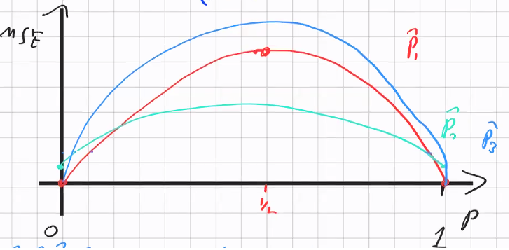
\includegraphics{images/MSE_Photo_2.png}
\end{center}
And so for different values of p we get different values of mean square error for each estimator and we might want to choose one over the either depending the values of p. 
\end{example}
\subsection{Unbiased Estimation}
You can see from the previous example that there is a trade-off between a low bias and low variance. For example to get the minimal variance you can just choose a constant regardless of the examples, yet this will tend to maximize the bias and so this isn't a good choice. On the other end you can minimize the bias (in absolute value) by taking the first sampling but this will tend to make the variance very large and so this isn't necessarily a good choice. This means that to get the best results for MSE there has to be some choice that will probably have non-zero bias and non-zero variance but that alltogether minimizes MSE. \\\\
Sometimes people still choose to focus on unbiased estimators. We will assume the existence of the expected value from now.
\begin{example}
Take $Y_1,\dots,Y_n\sim f_{\theta}(y)$ i.i.d. random variables with expected value $\mu$, and variance $\sigma^2$. Now we can ask whether or not the variance of the sample is an unbiased estimator for the variance. Where the variance of the sample is
\[\hat{\sigma^2}:=\frac{1}{n}\sum_{i=1}^n (Y_i-\bar{Y})^2\]
This means we need to calculate \[\mathbb{E}\left[\hat{\sigma^2}\right]= \mathbb{E}\left[\frac{1}{n}\sum_{i=1}^n (Y_i-\bar{Y})^2\right] = \frac{1}{n}\sum_{i=1}^n \left(\mathbb{E}\left[Y_i^2\right]\right)+\frac{1}{n}\mathbb{E}\left[\frac{-2Y_i}{n}\sum_i Y_i\right]+\frac{1}{n}\mathbb{E}\left[\sum_{i=1}^n \left(\frac{1}{n}\sum_i Y_i\right)\cdot \bar{Y}\right]=\]\[=\frac{1}{n}\sum_i\mathbb{E}\left[Y_i^2\right]-\frac{2}{n}\mathbb{E}\left[\sum_i Y_i\bar{Y}\right]+\frac{1}{n}\mathbb{E}\left[\sum_i Y_i\bar{Y}\right]=\frac{1}{n}\sum_i\mathbb{E}\left[Y_i^2\right] - \frac{1}{n}\mathbb{E}\left[\sum_i Y_i\bar{Y}\right]=\]\[=\frac{1}{n}\sum_i\mathbb{E}\left[Y_i^2\right]-\mathbb{E}\left[\bar{Y}^2\right]\]
Notice that \[\mathbb{E}\left[Y_i^2\right]=\sigma^2+\mu^2\]
And 
\[\mathbb{E}\left[\bar{Y}^2\right]=\frac{\sigma^2}{n}+\mu^2\]
And so 
\[\mathbb{E}[\hat{\sigma}^2]=\sigma^2+\mu^2-\frac{\sigma^2}{n}-\mu^2= \sigma^2\left(1-\frac{1}{n}\right)=\frac{n-1}{n}\sigma^2\]
We can now see that the sample variance isn't an unbiased estimator for the variance. Yet notice that the only thing that is preventing it from being unbiased is a multiplicative factor. To get an unbiased estimator for the variance we can then take
\[\hat{S^2}:=\frac{n}{n-1}\hat{\sigma}^2=\frac{\sum_i(Y_i-\bar{Y})^2}{n-1}\]
Notice though that this means that the variance was multiplied by $(\frac{n}{n-1})^2$, which again means we have a trade off between minimizing the variance and minimizing the bias. \end{example}
\textbf{Problem 6.1:} Assume that the expected value, $\mu$, is known and show that $\frac{1}{n}\sum_i (Y_i-\mu)^2$ is an unbiased estimator for $\sigma^2$. \\\\
Now we can ask the following question - Is there always an unbiased estimator for our values? Notice that uniqueness doesn't happen since we have seen that the sample average and the first sample are both unbiased estimators for the expected value. Now notice that if we have 2 unbiased estimators $\hat{\theta_1},\hat{\theta_2}$, then every convex sum $\alpha\hat{\theta_1}+(1-\alpha)\hat{\theta_2}$ is also an unbiased estimator. Now we will give an example where there isn't an unbiased estimator. \\\\
\begin{example}Take the bernoulli example - $Y_1,\dots,Y_n\sim\text{Be}(p)$, and look for an estimator for $\theta:=\frac{p}{1-p}$. Assume $\hat{\theta}$ is an estimator for $\theta$. And so 
\[\mathbb{E}[\hat{\theta}]=\sum_{y_1,\dots,y_n\in\{0,1\}^n} \hat{\theta}(\overrightarrow{y})p(\overrightarrow{y}) = \sum_{\overrightarrow{y}} \hat{\theta}(\overrightarrow{y})p^{\sum_i y_i}\cdot(1-p)^{n-\sum_i y_i}\]
This is a polynomial in p and $\theta$ doesn't have a full finite taylor polynomial expansion and so it cannot be estimated by an unbiased estimator and so this shows that there isn't always an unbiased estimator for every value. 
\end{example}
\subsection{Unbiased Estimator With Uniformly Minimal Variance}
\begin{definition} An estimator $\hat{\theta}$ is called an unbiased estimator with uniformly minimal variance (umvue) if it satisfies the following conditions\\\\
(1). $\hat{\theta}$ is an unbiased estimator.\\\\
(2). For any other unbiased estimator $\hat{\theta_1}$ 
\[\text{Var}(\hat{\theta})\leq\text{Var}(\hat{\theta_1})\]
For all $\theta\in\Theta$. \end{definition}
Notice that there isn't always a umvue since there isn't always an unbiased estimator. If though there is a umvue, then it is unique. 
\begin{proof}
For 2 umvue's $\hat{\theta_1},\hat{\theta_2}$, define $\hat{\theta}:=\frac{\hat{\theta{1}+\theta{2}}}{2}$. We get that
\[\text{Var}(\hat{\theta})=\frac{\text{Var}(\hat{\theta_1})+\text{Cov}(\hat{\theta_1},\hat{\theta_2})+\text{Var}(\hat{\theta_1})}{4}\leq\frac{\text{Var}(\hat{\theta_1})+2\sqrt{\text{Var}(\hat{\theta_1})\text{Var}(\hat{\theta_2})} + \text{Var}(\hat{\theta_2})}{4}\leq\]\[\leq\left(\frac{\sqrt{\text{Var}(\hat{\theta_1})}+\sqrt{\text{Var}(\hat{\theta_2})}}{2}\right)^2\leq \left(\max{\{\sqrt{\text{Var}(\hat{\theta_2})},\sqrt{\text{Var}(\hat{\theta_1})}\}}\right)^2\]
There is equality if and only if \[\sqrt{\text{Var}(\hat{\theta_2})} = \sqrt{\text{Var}(\hat{\theta_1})}\]
And \[\text{Cov}(\hat{\theta_1},\hat{\theta_2}) = 2\sqrt{\text{Var}(\hat{\theta_1})\text{Var}(\hat{\theta_2})}\]
From the second equation we know that they are a linear function of each other, yet they have the same variance and the same expected value which means that 
\[\hat{\theta_1}=\hat{\theta_2}\]
This proves uniqueness. (Almost surely)\\\\
Assuming there is a umvue, is this the best estimator? it turns out that the answer is no. \end{proof}
\end{document}